\documentclass[compress]{beamer}

\usepackage[brazil,portuguese]{babel}
\usepackage[utf8]{inputenc}
%\usepackage{caption}
%\usepackage{subcaption}
\usepackage{ragged2e}
\usepackage{graphicx}
\usepackage{tikz}
\usetikzlibrary{positioning}
\usetikzlibrary{decorations.pathreplacing}
\usetikzlibrary{decorations.pathmorphing}
\usetikzlibrary[patterns]
\usetikzlibrary{calc}
\usepackage{pgfplots}
\pgfplotsset{compat=newest}
\usepackage{amsfonts}
\usepackage{amssymb}
\usepackage{amsmath}
\usepackage{MnSymbol}
\usepackage[Algoritmo]{algorithm}
\usepackage[noend]{algorithmic}
\setbeamertemplate{bibliography entry title}{}
\setbeamertemplate{bibliography entry location}{}
\setbeamertemplate{bibliography entry note}{}

\newcounter{saveenumi}

\newcommand{\seti}{\setcounter{saveenumi}{\value{enumi}}}
\newcommand{\conti}{\setcounter{enumi}{\value{saveenumi}}}
\newtheorem{teorema}[theorem]{\scshape Teorema}
\newtheorem{proposicao}[theorem]{\scshape Proposição}
\newtheorem{corolario}[theorem]{\scshape Corolário}
\newtheorem{lema}[theorem]{\scshape Lema}
\newtheorem{definicao}[theorem]{\scshape Definição}
\newtheorem{conjectura}[theorem]{\scshape Conjectura}
\newtheorem{escolio}[theorem]{\scshape Escólio}
\newtheorem{exemplo}[theorem]{\scshape Exemplo}
\newtheorem{exemplos}[theorem]{\scshape Exemplos}
\newtheorem{propriedade}[theorem]{\scshape Propriedade}

\renewcommand{\u}{{\bf u}}
\renewcommand{\v}{{\bf v}}
\renewcommand{\sin}{\operatorname{sen}}
\renewcommand{\tan}{\operatorname{tg}}
\providecommand{\cas}{\operatorname{cas}}
\providecommand{\mdc}{\mathrm{mdc}}
\providecommand{\f}{{\bf f}}

\newcommand{\ie}{\textit{i.e.}}
\newcommand{\eg}{\textit{e.g.}}
\renewcommand\Re{\operatorname{Re}}
\renewcommand\Im{\operatorname{Im}}

\providecommand{\x}{{\bf x}}
\providecommand{\y}{{\bf y}}
\providecommand{\w}{{\bf w}}
\providecommand{\f}{{\bf f}}
\providecommand{\q}{{\bf q}}
\providecommand{\bfa}{{\bf a}}
\providecommand{\bfb}{{\bf b}}
\providecommand{\bfc}{{\bf c}}
\providecommand{\bfd}{{\bf d}}
\providecommand{\bfe}{{\bf e}}
\providecommand{\bfs}{{\bf s}}
\providecommand{\bfz}{{\bf z}}
\providecommand{\zero}{{\bf 0}}
\providecommand{\spn}{\mathrm{span}}
\providecommand{\posto}{\mathrm{posto}}
\providecommand{\nul}{\mathrm{nul}}
\providecommand{\proj}{\mathrm{proj}}
\providecommand{\tr}{\mathrm{tr}}
\providecommand{\sgn}{\mathrm{sgn}}
\providecommand{\cov}{\mathrm{cov}}
\providecommand{\dilation}{\mathcal{D}}
\providecommand{\erosion}{\mathcal{E}}
\providecommand{\open}{\mathcal{O}}
\providecommand{\close}{\mathcal{C}}

\newcommand*{\Bhat}{\skew{3}{\hat}{B}}

\mode<presentation>
{
  \setbeamertemplate{background canvas}[vertical shading][bottom=white!10,top=blue!10]
%  \usetheme{Berkeley}
%  \usetheme{CambridgeUS}
%  \usetheme{Madrid}
  \usetheme{Warsaw}
  \usefonttheme[onlysmall]{structurebold}  
  \setbeamertemplate{headline}{}  
% \setbeamercovered{invisible} % default
  \setbeamercovered{transparent, again covered={\opaqueness{25}} } % =15%
% \setbeamercovered{transparent=50}
% \setbeamercovered{dynamic}
% \setbeamercovered{again covered={\opaqueness<1->{25}}}
}

\usepackage{ifthen}
\makeatletter
\newcommand{\includecoveredgraphics}[2][]{
    \ifthenelse{\the\beamer@coveringdepth=1}{
        \tikz
            \node[inner sep=0pt,outer sep=0pt,opacity=0.15]
                {\includegraphics[#1]{#2}};
    }{
        \tikz
            \node[inner sep=0pt,outer sep=0pt]
                {\includegraphics[#1]{#2}};%
    }
} 
%\makeatother

%%% CAPA %%%
\title{Usando criptografia de forma prática e descomplicada}
\author{Marcos Azevedo aka psylinux}
\date{BSidesSP - Edição 0xF - Maio 2018 }


%%% APRESENTAÇÃO %%%
\begin{document}
\frame{\titlepage}

%%% SUMÁRIO %%%
%\section{Sumário}
%\frame{\tableofcontents}
%\section{}

\begin{frame}
\frametitle{Sumário}
	\begin{enumerate}
		\item<+->{Apresentação Pessoal}
		\item<+->{Qual a relevância desse tema?}
		\item<+->{História da Criptografia}
		\begin{enumerate}
			\item<+->{Cifra de César}
		\end{enumerate}
		\item<+->{Introdução à criptografia}
		\begin{enumerate}
			\item<+->{Definições e terminologias}
			\item<+->{Visão geral e funcionamento básico}
		\end{enumerate}
		\item<+->{Alguns tipos de criptografia}
		\begin{enumerate}
			\item<+->{Criptografia Simétrica}
			\item<+->{Criptografia Assimétrica}
			\item<+->{Assinatura Digital}
		\end{enumerate}
		\item<+->{Ferramentas para usar no dia-a-dia (Linux e Windows)}
		\begin{enumerate}
			\item<+->{GPG e PGP}
			\item<+->{Assinatura de Arquivo}
			\item<+->{Criptografia de Arquivos}
			\item<+->{Assinatura de E-mail}
			\item<+->{Criptografia em E-mail}
			\item<+->{Chave GPG para Login em SSH}
		\end{enumerate}
		\item<+->{Considerações finais}
	\end{enumerate}
\end{frame}

%\begin{frame}
%	{\tableofcontents}
%\end{frame}

%%% SLIDE %%%
\begin{frame}
\frametitle{Apresentação Pessoal}
	\justifying
		Marcos Azevedo - Consultor de Segurança na Cipher. Possui mais de 15 anos de experiência em Segurança da Informação, onde os últimos quatro anos foram dedicados a hardening de servidores, correção de problemas de segurança, análise forense, pentesting e segurança ofensiva. Ele tem um bom conhecimento de sistemas operacionais, arquitetura de computadores, compiladores e montadores para Intel x86, linguagem C, Python, PowerShell Scripts e Shell Scripts. Possui um sólido conhecimento de protocolos TCP/IP e experiência em infraestrutura de rede (Cisco Routers and Switches). Sua curva de aprendizado é muito rápida graças aos seus conhecimentos sólidos dos princípios da computação, além da motivação por desafios. Marcos já palestrou em conferências tais como: H2HC, FLISOL, FGSL e outros.
\end{frame}

%%% SLIDE %%%
\begin{frame}
\frametitle{Apresentação Pessoal}
	\begin{figure}[h]
		\caption{Goiânia, Goiás}
		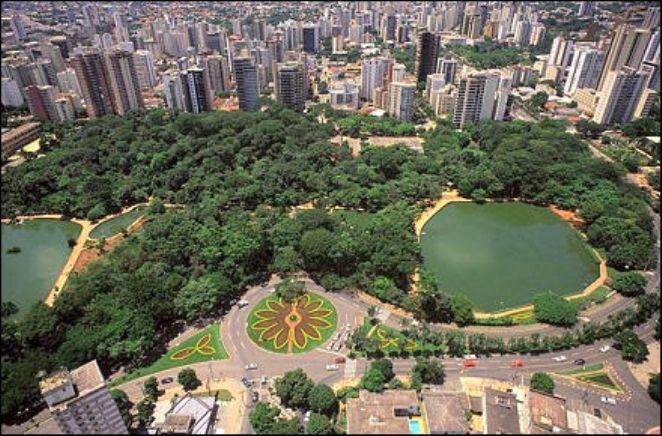
\includegraphics[width=\textwidth]{pics/goiania}
	\end{figure}
\end{frame}

%%% SLIDE %%%
\begin{frame}
\frametitle{Goianês ou Criptografia?}
	\begin{itemize}
		\justifying
		\item<+->{\textbf{Dinheiro pra sapecar porco}: Muito dinheiro.}
		\item<+->{\textbf{Custoso (a)}: Difícil, pessoa sapeca.}
		\item<+->{\textbf{Demais da conta}: Muito, muito mesmo.}
		\item<+->{\textbf{Encabulado}: Impressionado.}
		\item<+->{\textbf{Pizêro}: Bagunça.}
		\item<+->{\textbf{Pulá o corguim}: Passar dos limites.}
		\item<+->{\textbf{Apiar}: Descer.}
	\end{itemize}
\end{frame}

%%% SLIDE %%%
\begin{frame}
\frametitle{O que é Criptografia?}
\framesubtitle{Visão Geral}
\begin{figure}[h]
	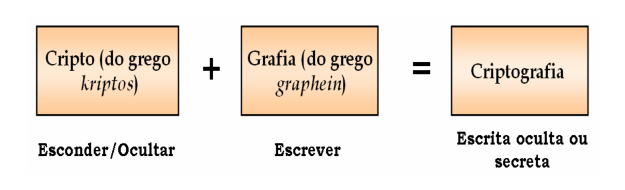
\includegraphics[width=\textwidth]{pics/cripto_1}
\end{figure}
\end{frame}

%%% SLIDE %%%
\begin{frame}
	\centering
	\textbf{"Criptografia"}\\
	\textbf{Qual a relevância desse tema?}
\end{frame}

%%% SLIDE %%%
\begin{frame}
	\frametitle{Qual a relevância desse tema?}
	\framesubtitle{Por que usamos criptografia?}
	\centering
		Quando queremos que apenas o \textbf{EMISSOR} e o \textbf{DESTINATÁRIO} compreendam o conteúdo da mensagem.
\end{frame}

%%% SLIDE %%%		
\begin{frame}
\frametitle{Qual a relevância desse tema?}
\framesubtitle{Quando usamos criptografia?}
	\begin{itemize}
		\justifying
		\item<+->{\textbf{"Em trânsito"}, neste contexto, é quando você envia informações através da Internet, por e-mail ou quando precisa armazená-la em outro lugar que não seja o seu próprio dispositivo.}
		\item<+->{\textbf{"Em repouso"}, quando estão armazenados em seu dispositivo, que pode ser parte integrada como um disco rígido, ou em um meio removível, como uma unidade USB.}
	\end{itemize}
\end{frame}

%%% SLIDE %%%		
\begin{frame}
\frametitle{Tipos de Algoritmos}
\begin{enumerate}
	\justifying
	\item<+->{\textbf{Criptografia Clássica:} Sustenta-se em leis matemáticas.}
	\item<+->{\textbf{Criptografia Quântica:} Utiliza-se de elementos físicos, tal com fótons, para gerar chaves quânticas inquebráveis.}
\end{enumerate}
\end{frame}

%%% SLIDE %%%		
\begin{frame}
\frametitle{Tipos de Algoritmos}
\framesubtitle{Criptografia Clássica}
\begin{enumerate}
	\justifying
	\item<+->{\textbf{Algoritmo de transposição:} rearranja a ordem dos caracteres de uma mensagem. Um exemplo simples é a transformação de \textbf{“muito obrigado”} em \textbf{“omtui oobdraig”}. Esta categoria de algoritmo criptográfico é composta por uma função bijetora	para efetuar encriptações e sua	inversa faz a mensagem voltar à forma original;}
	\item<+->{\textbf{Algoritmo de substituição:} substitui caracteres ou grupos de caracteres por outros caracteres ou grupos de caracteres. Um exemplo simples: \textbf{“muito obrigado”} é transformado em \textbf{“nvjup pcsjhbep”}, substituindo cada letra pela próxima na sequência alfabética.}
\end{enumerate}
\end{frame}

%%% SLIDE %%%
\begin{frame}
\frametitle{Entendendo o Algoritmo de Euclides}
\begin{figure}[h]
	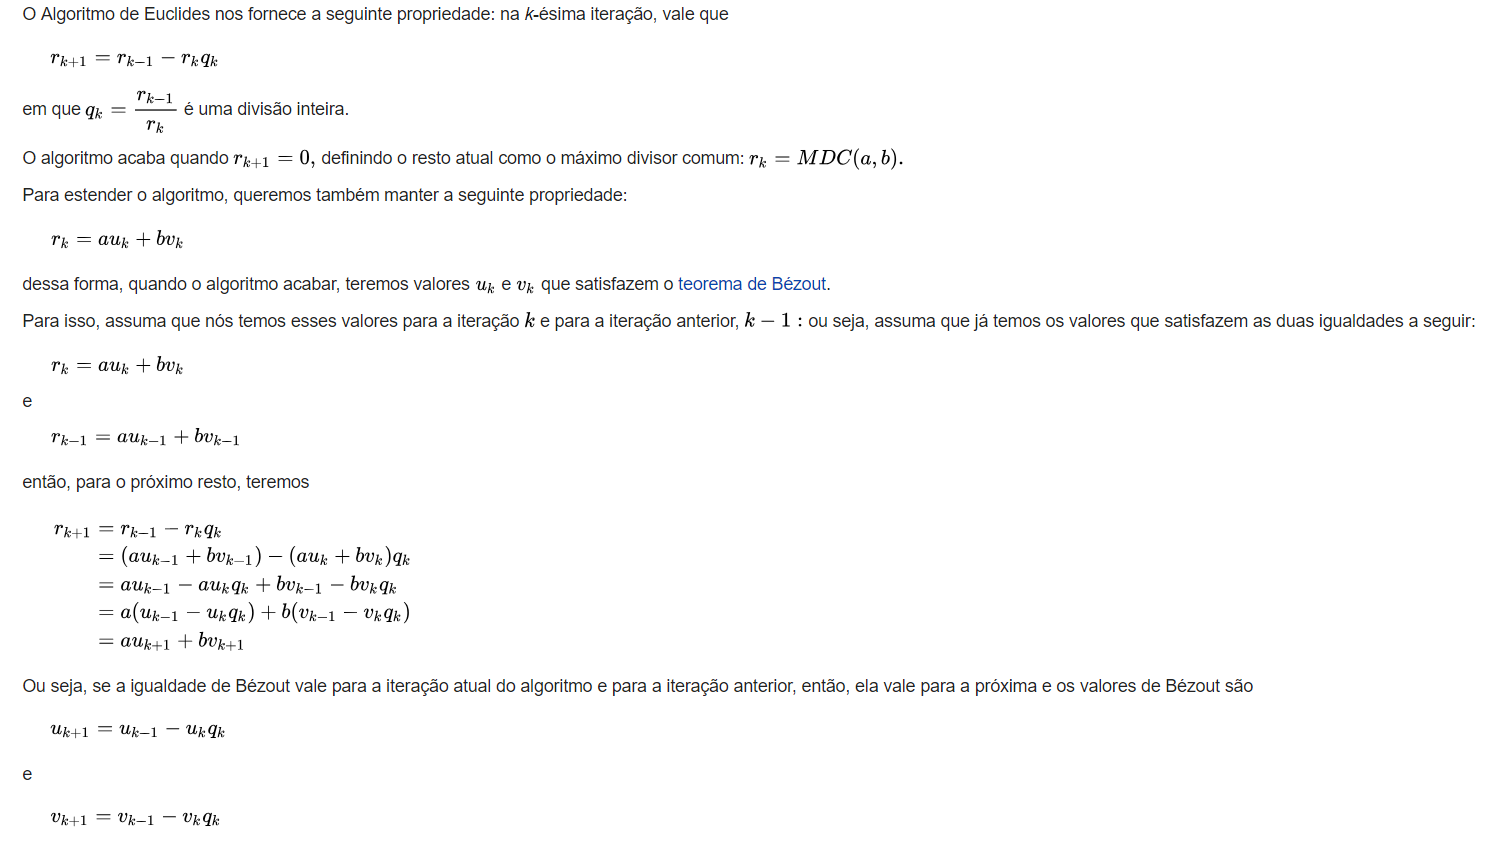
\includegraphics[width=\textwidth]{pics/euclides_1}
\end{figure}
\end{frame}

%%% SLIDE %%%
\begin{frame}
\frametitle{Criptografia Clássica}
\framesubtitle{Algoritmo de Transposição}
\centering
\textbf{{\LARGE BRINCADEIRA GENTE!}}
\end{frame}

%%% SLIDE %%%
\begin{frame}
\frametitle{Criptografia Clássica}
\framesubtitle{Algoritmo de Transposição}
\centering
Mensagem: \textbf{CRIPTOGRAFIA NA BSIDES SAO PAULO 2018}
\end{frame}

%%% SLIDE %%%		
\begin{frame}
\frametitle{Criptografia Clássica}
\framesubtitle{Algoritmo de Transposição}
	\begin{figure}[h]
		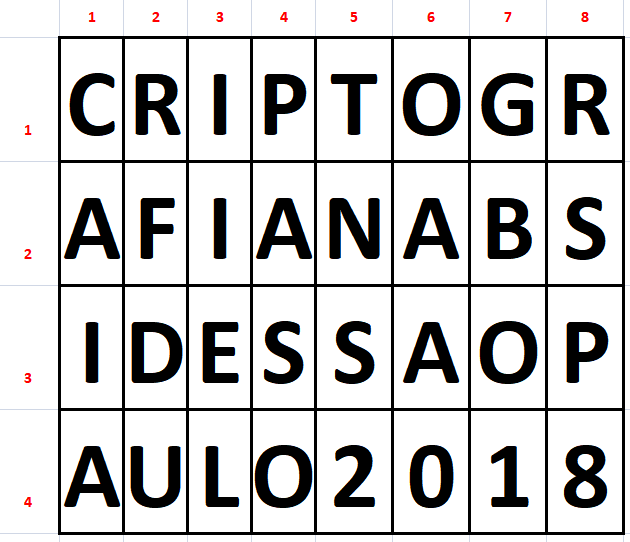
\includegraphics[width=\textwidth,height=7cm]{pics/tab_trans_1}
	\end{figure}
\end{frame}

%%% SLIDE %%%
\begin{frame}
\frametitle{Criptografia Clássica}
\framesubtitle{Algoritmo de Transposição}
\centering
Chave criptográfica: \textbf{24176835}
\end{frame}

%%% SLIDE %%%		
\begin{frame}
\frametitle{Criptografia Clássica}
\framesubtitle{Algoritmo de Transposição}
\begin{figure}[h]
	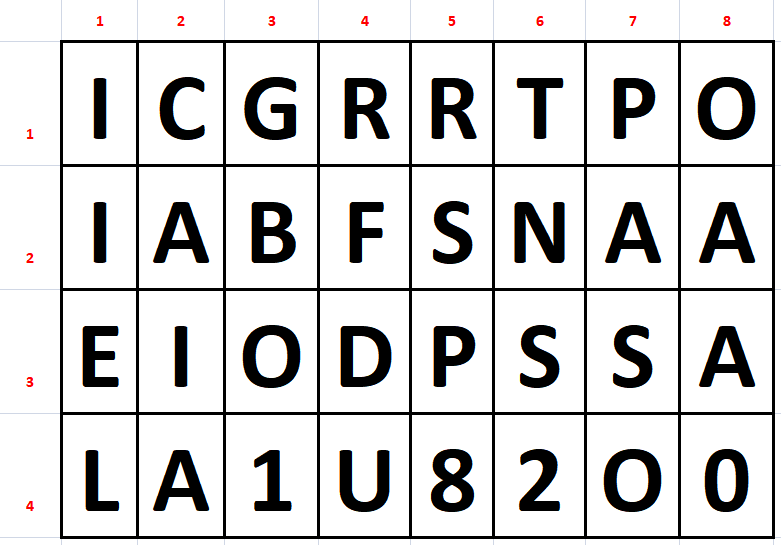
\includegraphics[width=\textwidth,height=7cm]{pics/tab_trans_2}
\end{figure}
\end{frame}

%%% SLIDE %%%		
\begin{frame}
\frametitle{Criptografia Clássica}
\framesubtitle{Algoritmo de Substituição}
\justifying
3M UM D14 D3 VER40, 3S7AVA N4 PR4I4,O853RV4NDO DU4S CR14NÇ4S 8B1NC4ND0 N4 4REI4. EL45 TR4B4LH4V4M MUI7O C0N57R1ND0 UM C4ATEL0 D3 AR3I4, C0M 70RR35, P4554R3L4S 3 P4554G3N5 1N7ERN4S. QU4ND0 ES74V4M QU4S3 T3RM1N4ND0, V310 UM4 0ND4 3 3S7RU1U 7UDO, R3DU21NDO 0 C4S7EL0 4 UM MON73 D3 4REI4 3 3SPUM4. 4CH31 QU3 D3P01S D3 74N70 35FORÇ0 3 CU1D4D0, 45 CR1ANC4S C4IR4M N0 CH0R0,
CORR3R4M P3L4 PR41A, FUG1ND0 DA 4GU4, R1NDO D3 M405 D4D4S 3 C0M3C4R4M 4 C0NS7RU1R 0UTR0 C4573LO. 
\end{frame}


%%% SLIDE %%%		
\begin{frame}
\frametitle{Algumas Aplicações da Criptografia Atualmente}
		\begin{enumerate}
			\item{Sigilo em banco de dados;}
			\item{Censos;}
			\item{Investigações governamentais;}
			\item{Dossiês de pessoas sob investigação;}
			\item{Dados hospitalares;}
			\item{Informações de crédito pessoal;}
			\item{Decisões estratégicas empresariais;}
			\item{Sigilo em comunicação de dados;}
			\item{Comandos militares;}
			\item{Mensagens diplomáticas;}
			\item{Operações bancárias;}
			\item{Comércio eletrônico;}
			\item{Transações por troca de documentos eletrônicos (EDI);}
			\item{Estudo de idiomas desconhecidos;}
			\item{Recuperação de documentos arqueológicos, hieróglifos;}
			\item{E até tentativas de comunicações extraterrestres.}
		\end{enumerate}
\end{frame}

%%% SLIDE %%%		
\begin{frame}
\frametitle{Introdução à Criptografia}
\framesubtitle{Definições e terminologias | Criptologia}
\justifying
	\textbf{Criptologia:} disciplina que reúne os conhecimentos e as técnicas necessários à criptoanálise ('solução de criptogramas') e à criptografia ('modificação codificada').
\end{frame}

%%% SLIDE %%%		
\begin{frame}
\frametitle{Introdução à Criptografia}
\framesubtitle{Definições e terminologias | Texto Claro}
\justifying
\textbf{Texto Claro:} Texto original, não cifrado.
\end{frame}

%%% SLIDE %%%		
\begin{frame}
\frametitle{Introdução à Criptografia}
\framesubtitle{Definições e terminologias | Texto Cifrado}
\justifying
\textbf{Texto Cifrado:} Texto ilegível, não compreensível.
\end{frame}

%%% SLIDE %%%		
\begin{frame}
\frametitle{Introdução à Criptografia}
\framesubtitle{Definições e terminologias | Simetria}
\justifying
	\textbf{Simetria:} conformidade, em medida, forma e posição relativa, entre as partes dispostas em cada lado de uma linha divisória, um plano médio, um centro ou um eixo
\end{frame}

%%% SLIDE %%%		
\begin{frame}
\frametitle{Introdução à Criptografia}
\framesubtitle{Definições e terminologias | Assimetria}
\justifying
	\textbf{Assimetria:} 1. ausência de simetria. 2. grande diferença; disparidade, discrepância
\end{frame}

%%% SLIDE %%%		
\begin{frame}
\frametitle{Introdução à Criptografia}
\framesubtitle{Definições e terminologias | Encriptar/Cifrar}
\justifying
	\textbf{Encriptar/Cifrar:} 1. reproduzir (mensagem) em código não conhecido, tornando-a, desse modo, intencionalmente ininteligível para os que não têm acesso às suas convenções. 2. inf codificar (informação) de modo que somente destinatários autorizados possam ter acesso a ela; encriptar.
\end{frame}

%%% SLIDE %%%		
\begin{frame}
\frametitle{Introdução à Criptografia}
\framesubtitle{Definições e terminologias | Decriptar/Decifrar}
\justifying
	\textbf{Decriptar/Decifrar:} traduzir ou decifrar mensagens ou códigos cifrados ou criptografados
\end{frame}

%%% SLIDE %%%		
\begin{frame}
\frametitle{Introdução à Criptografia}
\framesubtitle{Definições e terminologias | Bit}
\justifying
	\textbf{Bit:} menor parcela de informação processada por um computador. Algarismo do sistema binário que somente pode assumir as formas 0 ou 1
\end{frame}

%%% SLIDE %%%		
\begin{frame}
\frametitle{Introdução à Criptografia}
\framesubtitle{Definições e terminologias | Algoritmo}
\justifying
	\textbf{Algoritmo:} 1. mat sequência finita de regras, raciocínios ou operações que, aplicada a um número finito de dados, permite solucionar classes semelhantes de problemas. 2. inf conjunto das regras e procedimentos lógicos perfeitamente definidos que levam à solução de um problema em um número finito de etapas.
\end{frame}

%%% SLIDE %%%
\begin{frame}
\frametitle{O Princípio de Kerckhoff}
	\center
	O Princípio de Kerckhoff é um princípio fundamental na criptografia moderna: \\
	\textbf{"Um sistema de criptografia deve ser seguro mesmo se o adversário conhecer todos os detalhes do sistema, com exceção da chave secreta."}
\end{frame}

%%% SLIDE %%%
\begin{frame}
\frametitle{Algoritmos Cifradores}
\justifying
\begin{enumerate}
	\item<+->{\textbf{Cifradores de blocos:} divide a mensagem
		em blocos de tamanho fixo (ex: 256 bits). Por exemplo, DES, AES, 3DES}
	\item<+->{\textbf{Cifradores de fluxo:} cifra cada digito do texto plano por vez. Por exemplo, o RC4}
\end{enumerate}
\end{frame}

%%% SLIDE %%%
\begin{frame}{Alguns tipos de Chaves Criptograficas}
		\begin{enumerate}
			\item<+->{Criptografia Simétrica}
			\item<+->{Criptografia Assimétrica}
		\end{enumerate}
\end{frame}

%%% SLIDE %%%
\begin{frame}
\frametitle{Criptografia Simétrica}
\begin{enumerate}
	\item<+->{Também conhecido como: criptografia de chave única, criptografia de chave secreta.}
	\item<+->{A chave precisa ser transmitida através de um canal seguro.}
	\item<+->{Transmissão Wireless utilizam esse modelo criptográfico.}
\end{enumerate}
\end{frame}

%%% SLIDE %%%
\begin{frame}
\frametitle{Criptografia Assimétrica}
\begin{enumerate}
	\item<+->{Baseado no par de chaves: \textbf{pública e privada}}
	\begin{itemize}
		\item<+->{Chaves públicas são divulgadas abertamente.}
		\item<+->{Chaves privadas devem ser mantidas em segredo.}
		\item<+->{Não é possível obter a chave privada a partir da pública!}
	\end{itemize}
	\item<+->{Provê:}
	\begin{itemize}
		\item<+->{Confidencialidade das mensagens.}
		\item<+->{Autenticação do remetente.}
		\item<+->{Verificação de integridade.}
		\item<+->{Não repudio.}
	\end{itemize}
\end{enumerate}
\end{frame}


%%% SLIDE %%%		
\begin{frame}
\frametitle{Ferramentas para usar no dia-a-dia (Linux e Windows)}
		\begin{enumerate}
			\item<+->{GPG e PGP}
			\item<+->{Assinatura de Arquivo}
			\item<+->{Criptografia de Arquivos}
			\item<+->{Assinatura de E-mail}
			\item<+->{Criptografia em E-mail}
			\item<+->{Chave GPG para Login em SSH}
		\end{enumerate}
\end{frame}

%%%% SLIDE %%%		
\begin{frame}
\frametitle{Lições Aprendidas}
\justifying
	\begin{enumerate}
		\item<+->{Nunca, jamais, desenvolva o seu próprio algoritmo de criptografia, a menos que você tenha uma equipe de experientes criptoanalistas verificando o seu projeto.}
		\item<+->{Não utilize algoritmos de criptografia não comprovados ou protocolos não comprovados.}
		\item<+->{Os atacantes vão sempre olhar para o ponto mais fraco de um sistema de criptografia. Por exemplo, um grande espaço de chaves por si só não é garantia de uma cifra segura; a cifra ainda pode estar vulnerável contra ataques analíticos.}
	\end{enumerate}
\end{frame}

%%%% SLIDE %%%		
\begin{frame}
\frametitle{Lições Aprendidas}
\justifying
	\begin{enumerate}
		\setcounter{enumi}{3}
		\item<+->{Comprimentos de chave de algoritmos simétricos, a fim de frustrar ataques de busca exaustiva da chave:}
		\begin{itemize}
			\item<+->{64 bits: inseguro exceto para dados cujo uso se dará num prazo muito curto.}
			\item<+->{128 bits: segurança de longo prazo para várias décadas, a menos que os computadores quânticos se tornem disponíveis (computadores quânticos não existem e talvez nunca existam).}
			\item<+->{256 bits: como acima, mas provavelmente seguros até contra ataques por computadores quânticos.}
			\item<+->{Aritmética modular é uma ferramenta para exprimir os esquemas de encriptação históricos, tais como a Cifra Afim, de uma maneira matematicamente elegante.}
		\end{itemize}
	\end{enumerate}
\end{frame}

%%%% SLIDE %%%		
\begin{frame}{Considerações Finais}
\end{frame}

%%% BIBLIOGRAFIA %%%
%\begin{frame}[allowframebreaks]
	%%\usepackage[fixlanguage]{babelbib}
	%%\selectbiblanguage{brazil}
	%\frametitle{Referências}
	%\bibliographystyle{plain}
	%\bibliography{bibliografia}
%\end{frame}

\end{document}

